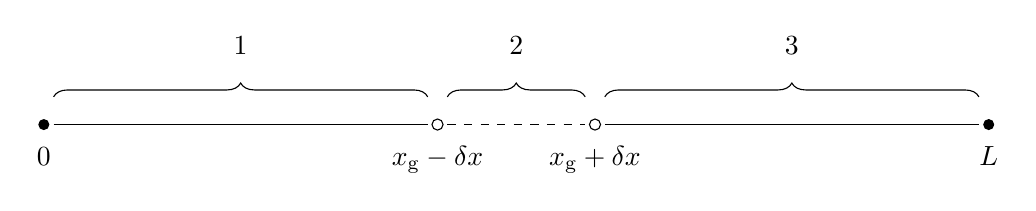
\begin{tikzpicture}
  \def\labelshift{(0, -0.4)}%
  \def\regionshift{(0, 1)}%
  \node[label={[anchor=base,shift=\labelshift]below:0}] (A) at (0, 0) {};
  \node[label={[anchor=base,shift=\labelshift]below:$x_{\mathrm{g}}-\delta x$}] (B) at (5, 0) {};
  \node[label={[anchor=base,shift=\labelshift]below:$x_{\mathrm{g}}+\delta x$}] (C) at (7, 0) {};
  \node[label={[anchor=base,shift=\labelshift]below:$L$}] (D) at (12, 0) {};

  \fill (A) circle (2pt) (D) circle (2pt);
  \draw (B) circle (2pt) (C) circle (2pt);
  \draw (A) -- (B) (C) -- (D);
  \draw[dashed] (B) -- (C);

  \draw[decorate,decoration={brace,amplitude=5pt,raise=10pt}] (A) -- (B) node[midway,shift=\regionshift]{1};
  \draw[decorate,decoration={brace,amplitude=5pt,raise=10pt}] (B) -- (C) node[midway,shift=\regionshift]{2};
  \draw[decorate,decoration={brace,amplitude=5pt,raise=10pt}] (C) -- (D) node[midway,shift=\regionshift]{3};
\end{tikzpicture}
